\section{Theoretical Peak Performance of CPU}

\begin{figure}
    \centering
    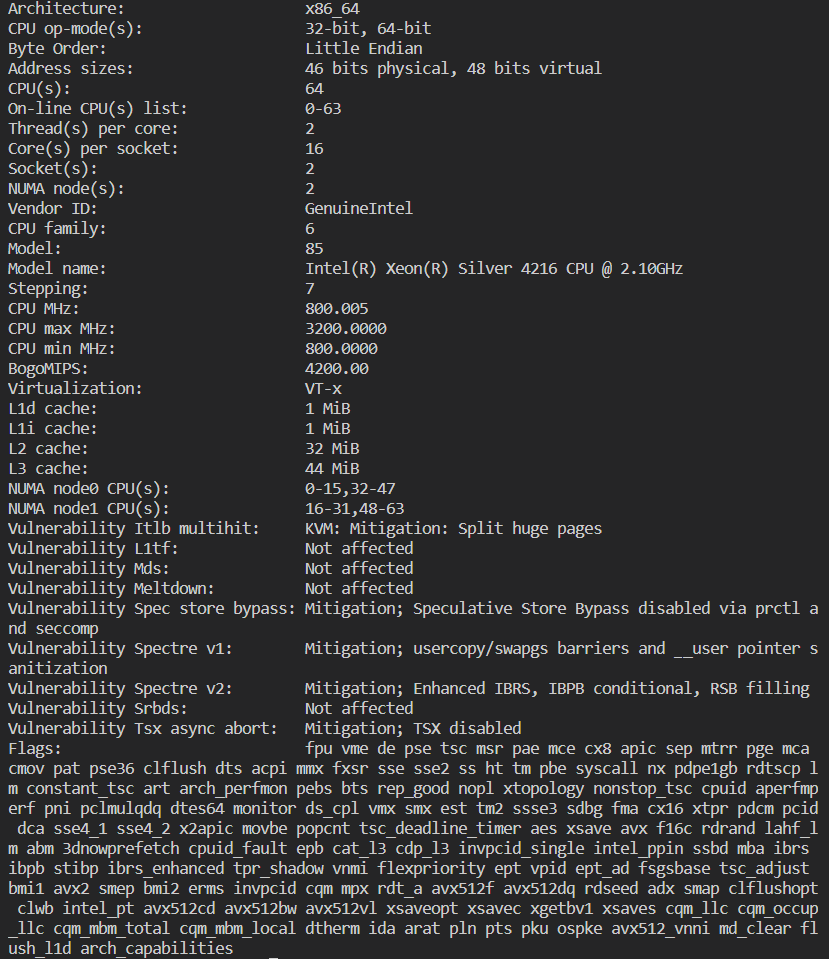
\includegraphics[scale=0.8]{imgs/lscpu.png}
    \caption{\label{fig:lscpu}
        계산 노드에서의 \texttt{lscpu} 명령어의 출력 결과.
    }
\end{figure}

Fig.~{\ref{fig:lscpu}}과 같이 계산 노드의 CPU 정보를 얻었다.

\begin{enumerate}[label= (\alph*)]

    \item {Intel(R) Xeon(R) Silver 4216 CPU @ 2.10GHz}
    \item {2개의 CPU가 장착되어 있다.}
    \item {
        Base clock frequency는 2.10GHz이고, boost clock frequency는 3.20 GHz이다.
        Base clock과 boost clock은 각각 CPU가 동작할 수 있는 최소, 최대의 clock을 의미하며,
        CPU는 현재 수행중인 workload가 필요로 하는 연산 성능을 판단하여 clock speed를 조정한다.
        이 때 clock speed를 조정하는 범위를 base clock과 boost clock으로 제한한다.
        CPU가 boost clock frequency로 동작하기 위한 조건으로는, 현재 수행중인 workload가 높은 성능을 필요로 하고,
        공급되는 전력이 충분하며, CPU의 온도가 너무 높지 않아야 한다.
    }
    \item {
        하나의 CPU에서 physical core는 16개, logical core는 32개이다.
        Theoretical peak performance 계산을 위해서는 physical core 개수인 16를 사용해야 하며,
        그 이유는 logical core는 하나의 physical core가 동시에 여러 thread를 연산할 수 있도록 하는
        기술(i.e. Hyper-Threading, SMT 등)을 적용하여 얻어진 가상의 개념이므로,
        실제 연산의 성능은 결국 physical core에 달려 있기 때문이다.
        
    }
    \item {
        Intel(R) Xeon(R) Silver 4216 CPU 는 1개의 AVX512 FMA 유닛을 갖고 있다.
        이를 바탕으로 한 clock cycle당 실행되는 AVX512 instruction의 수는 1개라고 가정하자.
        AVX512 instruction 하나가 수행할 수 있는 FP32 연산의 수는 $512/32=16$개이다.
        따라서 하나의 core가 한 clock cycle에 수행할 수 있는 FP32 연산의 수는 16개이다.
    }
    \item {
        Theoretical peak performance를 다음과 같이 계산할 수 있다.
        
        \begin{align}
            R_{peak}
            & =     \mathrm{\frac{(\#~of~FP32~operation)}{(\#~of~core)(\#~of~clock)}}
            \times  \mathrm{(\#~of~core)}
            \times  \mathrm{(boost~clock~frequency)} \notag \\
            & = 16 \times 3.2 \times 32 \notag \\
            & = {1638.4}~\mathrm{(GFLOPS)} \notag
        \end{align}
    
    }
    
\end{enumerate}